% Provenance (never printed): see sources/outline_sources.md (Year 1:
% astronomy of position, spherical trigonometry, time scales, insolation).
% Spherical trigonometry is absent from the mathematics series: this chapter
% owns it. Curves computed in figdata/bachelor-1/{sun_paths, day_length,
% celestial_sphere, spherical_triangle}.py (shared model _solar.py); numbers
% of the exercises and problem in the Book 3 scratch calculator ch01.py.
\chapter{الفلك الكروي}\label{ch:b1:spherical-astronomy}

في ليلة صافية بعيدًا عن أي مدينة، تُسجّل كاميرا ذات تعريض طويل موجّهة نحو السماء النجومَ أقواسًا من دوائر، كلها متمركزة حول نقطة واحدة لا تتحرك. فالنجم الذي طلع من الشرق عند التاسعة من هذه الليلة يطلع غدًا قرابة التاسعة إلا خمس دقائق، ثم يطلع أبكر فأبكر كل ليلة بعدها. والشمس عند الظهر أعلى في يونيو منها في ديسمبر، وفي أقصى الشمال لا تغيب البتة في منتصف الصيف. كل ذلك ناتج عن دوران الأرض حول محورها وعن دورانها حول الشمس، كما يبدو من سطحها. ولوصف ذلك يحتاج الفلكي والجيولوجي إلى إحداثيات على كرة، وإلى مثلثات مرسومة على الكرة، وإلى ساعات تتبع النجوم أو الشمس. وهذا الفصل يبني هذه الأدوات. وتعود في حركيات الصفائح (\cref{ch:b1:plate-kinematics})، حيث تدور الصفائح على الكرة، وفي فصول المناخ (\cref{ch:b1:radiation-heat-transport})، حيث يحرّك ضوء الشمس الذي تتلقاه كل بقعة بحسب عرضها الجغرافي الرياحَ والتيارات.

\begin{recall}
تدور الأرض حول محورها مرةً في اليوم، وتدور حول الشمس مرةً في السنة على مدار يكاد يكون دائريًا؛ ومحورها مائل على مستوى هذا المدار، وهذا \omterm{def:b1:spherical-astronomy:equatorial}{الميل} هو ما يصنع الفصول (كتب الفيزياء، الصف 6 والصف 12؛ وتُستعاد قوانين كبلر من كتاب الفيزياء للسنة الأولى). وتُحدَّد نقطة على الأرض بعرضها الجغرافي وطولها الجغرافي (الكتاب 1، الصف 6). ومتجهة طولها واحد تتعيّن بزاويتين، كما في الإحداثيات الكروية؛ والجداء السلّمي لمتجهتين وحدويتين هو جيب تمام الزاوية بينهما، والجداء المختلط $\vec u\cdot(\vec v\times\vec w)$ لا يتغيّر بالتبديل الدوري للمتجهات الثلاث.
\end{recall}

\section{المثلثات على الكرة}

\begin{definition}[الدائرة العظمى، المثلث الكروي]\label{def:b1:spherical-astronomy:spherical-triangle}
\emph{الدائرة العظمى}\index{الدائرة العظمى} لكرة هي تقاطعها مع مستوٍ يمرّ بمركزها؛ وكل مقطع آخر بمستوٍ يسمّى \emph{دائرة صغرى}\index{الدائرة الصغرى}. وعبر نقطتين غير متقابلتين قطريًا تمرّ دائرة عظمى واحدة وحدها، وأقصر قوسيها هو أقصر طريق بين النقطتين على الكرة. و\emph{المثلث الكروي}\index{المثلث الكروي} هو الشكل الذي تكوّنه ثلاث نقاط على الكرة، هي رؤوسه $A$ و$B$ و$C$، تصلها أقواس من دوائر عظمى أقصر من \ang{180}. وأضلاعه $a$ و$b$ و$c$ المقابلة للرؤوس $A$ و$B$ و$C$ على الترتيب تُقاس بالزوايا التي تحصرها عند المركز، وزواياه $A$ و$B$ و$C$ هي الزوايا بين مستويي الضلعين اللذين يلتقيان عند كل رأس.
\end{definition}

على كرة نصف قطرها $R$ يكون للضلع الذي طوله $a$ راديانًا الطولُ $Ra$. وكل ضلع وكل زاوية محصوران بين $0$ و$\pi$.

\begin{omfigure}
\begin{tikzpicture}
\begin{axis}[x=1cm, y=1cm, hide axis, xmin=-2.7, xmax=2.7, ymin=-2.6, ymax=2.6, clip=false]
\draw[black, line width=0.6pt] (axis cs:0,0) circle (2.4cm);
\addplot[black!45, densely dashed, line width=0.4pt] coordinates {(0,0) (-0.078358,1.7847)};
\addplot[black!45, densely dashed, line width=0.4pt] coordinates {(0,0) (-1.5903,-0.2902)};
\addplot[black!45, densely dashed, line width=0.4pt] coordinates {(0,0) (1.4453,-0.16381)};
\addplot[omDef, line width=1.1pt] table {figdata/out/bachelor-1-spherical_triangle-ab.dat};
\addplot[omDef, line width=1.1pt] table {figdata/out/bachelor-1-spherical_triangle-bc.dat};
\addplot[omDef, line width=1.1pt] table {figdata/out/bachelor-1-spherical_triangle-ca.dat};
\addplot[omThm, line width=0.8pt] table {figdata/out/bachelor-1-spherical_triangle-angA.dat};
\addplot[only marks, mark=*, mark size=1.4pt] table[x=x, y=y] {figdata/out/bachelor-1-spherical_triangle-verts.dat};
\fill (axis cs:0,0) circle (1.2pt);
\begin{scope}[font=\small]
  \node[above] at (axis cs:-0.078358,1.7847) {$A$};
  \node[left] at (axis cs:-1.5903,-0.2902) {$B$};
  \node[right] at (axis cs:1.4453,-0.16381) {$C$};
  \node[above left] at (axis cs:0,0) {$O$};
  \node[omThm] at (axis cs:0.24,1.36) {$A$};
  \node[omDef] at (axis cs:0.0,-0.52) {$a$};
  \node[omDef] at (axis cs:0.95,0.95) {$b$};
  \node[omDef] at (axis cs:-1.05,0.95) {$c$};
\end{scope}
\end{axis}
\end{tikzpicture}

{\small مثلث كروي $ABC$ على كرة مركزها $O$. أضلاعه $a$ و$b$ و$c$ أقواس من دوائر عظمى، تُقاس بالزاويتين $BOC$ و$COA$ و$AOB$؛ والزاوية $A$ (بالأحمر) هي الزاوية بين الضلعين اللذين يلتقيان عند $A$. والمثلث المرسوم فيه $a = \ang{78.6}$ و$b = \ang{62.6}$ و$c = \ang{64.8}$، وزواياه \ang{89.9} و\ang{64.9} و\ang{67.4}، ومجموعها أكبر من \ang{180}.}
\end{omfigure}

\begin{theorem}[قاعدة جيب التمام]\label{thm:b1:spherical-astronomy:cosine-rule}
في \omterm{def:b1:spherical-astronomy:spherical-triangle}{المثلث الكروي}،
\[
  \cos a = \cos b\cos c + \sin b\sin c\cos A .
\]
\end{theorem}

\begin{proof}
نعمل على الكرة الوحدوية، ونختار المحاور بحيث تقع $A$ عند القطب:
$\vec A = (0, 0, 1)$، والمستوي $xz$ الذي يحوي $B$:
$\vec B = (\sin c, 0, \cos c)$، لأن $B$ تبعد بالزاوية $c$ عن النقطة $A$.
والنقطة $C$ تبعد بالزاوية $b$ عن $A$، وتقع على دائرة عظمى تمرّ بالنقطة $A$ وتصنع الزاوية $A$ مع المستوي $xz$:
$\vec C = (\sin b\cos A, \sin b\sin A, \cos b)$. والضلع $a$ هو الزاوية بين $\vec B$ و$\vec C$، إذن
\[
  \cos a = \vec B\cdot\vec C = \sin c\sin b\cos A + \cos c\cos b. \qedhere
\]
\end{proof}

\begin{theorem}[قاعدة الجيب]\label{thm:b1:spherical-astronomy:sine-rule}
في \omterm{def:b1:spherical-astronomy:spherical-triangle}{المثلث الكروي}،
\[
  \frac{\sin A}{\sin a} = \frac{\sin B}{\sin b} = \frac{\sin C}{\sin c}.
\]
\end{theorem}

\begin{proof}
بالمتجهات الواردة في البرهان السابق، نحسب
$\vec B \times \vec C = (-\cos c\sin b\sin A,\ \cos c\sin b\cos A - \sin c\cos b,\
\sin c\sin b\sin A)$، فيكون الجداء المختلط
$\vec A\cdot(\vec B\times\vec C) = \sin b\sin c\sin A$. ولا يتغيّر الجداء المختلط بالتبديل الدوري للرؤوس $A$ و$B$ و$C$، وبوضع $B$ ثم $C$ عند القطب نحصل بالطريقة نفسها على $\sin c\sin a\sin B$ و$\sin a\sin b\sin
C$. والعبارات الثلاث متساوية؛ وبقسمتها على $\sin a\sin b\sin c$ نحصل على القاعدة.
\end{proof}

عندما تكون الأضلاع صغيرة بالنسبة إلى نصف القطر، يكون $\cos a \approx 1 -
a^2/2$ و$\sin a \approx a$، فتصير القاعدتان قاعدتي جيب التمام والجيب في المثلثات المستوية: فعلى رقعة صغيرة بما يكفي تكون الكرة مستوية. أما في المثلث الكبير فلا: فمجموع زوايا \omterm{def:b1:spherical-astronomy:spherical-triangle}{المثلث الكروي} أكبر من \ang{180} (\cref{exo:b1:spherical-astronomy:12}).

\begin{method}[حساب المسافة والاتجاه على الكرة]\label{met:b1:spherical-astronomy:great-circle}
لإيجاد أقصر مسافة بين موضعين عرضهما الجغرافي $\varphi_1$ و$\varphi_2$ وطولهما الجغرافي $\lambda_1$ و$\lambda_2$، والاتجاه الذي يُنطلق فيه:
\begin{enumerate}
  \item نكوّن المثلث الذي رؤوسه القطب الشمالي $P$ والموضعان؛ أضلاعه الخارجة من القطب هي متممات العرض $\ang{90} -
        \varphi_1$ و$\ang{90} - \varphi_2$، وزاويته عند القطب هي فرق \omterm{def:b1:spherical-astronomy:geographic}{الطول الجغرافي} $\Delta\lambda$؛
  \item تعطي قاعدة جيب التمام البعد الزاوي $\Delta$:
        $\cos\Delta = \sin\varphi_1\sin\varphi_2 +
        \cos\varphi_1\cos\varphi_2\cos\Delta\lambda$؛ والمسافة هي
        $R\Delta$ ($\Delta$ بالراديان)؛
  \item الاتجاه الابتدائي هو زاوية المثلث عند الموضع الأول، من قاعدة جيب التمام المطبّقة على الضلع المقابل لها،
        $\sin\varphi_2 = \sin\varphi_1\cos\Delta + \cos\varphi_1\sin\Delta\cos
        \mathrm{Az}$، ويُقاس من الشمال نحو الموضع الثاني.
\end{enumerate}
يتغيّر الاتجاه على طول \omterm{def:b1:spherical-astronomy:spherical-triangle}{الدائرة العظمى} (إلا على خط زوال أو على خط الاستواء): فالسفينة أو الطائرة التي تحافظ على الاتجاه نفسه في البوصلة تسلك منحنى آخر أطول.
\end{method}

\section{الإحداثيات على الكرة}

\begin{definition}[خط العرض وخط الطول]\label{def:b1:spherical-astronomy:geographic}
لتكن الأرض كرة تدور حول محورها القطبي. و\emph{العرض الجغرافي}\index{العرض الجغرافي} $\varphi$ لنقطة هو الزاوية بين مستوى خط الاستواء والنصف القطري المار بالنقطة، وتتراوح من \ang{-90}
(القطب الجنوبي) إلى \ang{+90} (القطب الشمالي)؛ و\emph{الطول الجغرافي}\index{الطول الجغرافي} $\lambda$ هو الزاوية، المقاسة في مستوى خط الاستواء، بين نصف مستوى الزوال المار بالنقطة ونصف مستوى زوال مرجعي، هو الزوال المار بغرينتش، وتُعدّ موجبة نحو الشرق، وتتراوح من \ang{-180} إلى \ang{180}.
\end{definition}

الأرض في الواقع مفلطحة قليلًا؛ والعرض المستعمل في الخرائط وفي السماء هو الزاوية بين الشاقول المحلي ومستوى خط الاستواء، وهو يختلف عن الزاوية المركزية بما لا يتجاوز \ang{0.2} (\cref{ch:b1:isostasy-gravity}). \omterm{def:b1:spherical-astronomy:geographic}{وخطوط العرض} المتساوي، أي دوائر العرض المتوازية، هي دوائر صغرى؛ أما خطوط الزوال فهي أنصاف دوائر عظمى.

\begin{definition}[الكرة السماوية]\label{def:b1:spherical-astronomy:celestial-sphere}
\emph{الكرة السماوية}\index{الكرة السماوية} كرة وهمية مركزها الراصد، تُوضع عليها كل نجمة في اتجاهها؛ والاتجاهات وحدها تهمّ لا المسافات. ويلتقي امتدادا محور الأرض بها عند \emph{القطبين السماويين}\index{القطب السماوي}، الشمالي والجنوبي؛ ومستوى خط استواء الأرض يقطعها على طول \emph{خط الاستواء السماوي}\index{خط الاستواء السماوي}. و\emph{سمت الرأس}\index{سمت الرأس} هو النقطة الواقعة فوق الراصد مباشرة على الشاقول المحلي؛ والأفق هو \omterm{def:b1:spherical-astronomy:spherical-triangle}{الدائرة العظمى} التي تبعد عنه $\ang{90}$. و\emph{خط الزوال المحلي}\index{خط الزوال المحلي} هو \omterm{def:b1:spherical-astronomy:spherical-triangle}{الدائرة العظمى} المارّة بسمت الرأس وبالقطبين السماويين؛ وهو يلتقي بالأفق عند نقطتي الشمال والجنوب.
\end{definition}

ولأن الأرض تدور من الغرب إلى الشرق، تبدو \omterm{def:b1:spherical-astronomy:celestial-sphere}{الكرة السماوية} كأنها تدور في الاتجاه المعاكس، من الشرق إلى الغرب، حول محور \omterm{def:b1:spherical-astronomy:celestial-sphere}{القطبين السماويين}، دورةً كاملةً في أقلّ قليلًا من يوم. وتحتفظ النجوم بمواضعها النسبية، فهي بعيدة إلى حدّ أن رحلة الأرض السنوية حول الشمس لا تغيّر اتجاهاتها إلا بأقلّ من ثانية قوسية (\cref{ch:b1:observing-the-sky}).

\begin{definition}[الإحداثيات الأفقية]\label{def:b1:spherical-astronomy:horizontal}
\emph{الارتفاع}\index{الارتفاع (للنجم)} $h$ للنجم هو زاويته فوق الأفق، وتتراوح من \ang{-90} إلى \ang{90}؛ وبُعده الزاوي عن \omterm{def:b1:spherical-astronomy:celestial-sphere}{سمت الرأس} هو $z = \ang{90} - h$. و\emph{السمت}\index{السمت} $\mathrm{A}$ هو الزاوية، على طول الأفق، من نقطة الشمال إلى أسفل دائرة الارتفاع المارّة بالنجم، وتُقاس من \ang{0} إلى \ang{360} مارّةً بالشرق.
\end{definition}

الإحداثيات الأفقية هي إحداثيات الراصد: تتغيّر بتغيّر المكان والزمن. أما إحداثيات السماء ذاتها فتدور معها بدوران \omterm{def:b1:spherical-astronomy:celestial-sphere}{الكرة السماوية}.

\begin{definition}[الإحداثيات الاستوائية]\label{def:b1:spherical-astronomy:equatorial}
\emph{الميل}\index{الميل (الفلكي)} $\delta$ للنجم هو زاويته عن \omterm{def:b1:spherical-astronomy:celestial-sphere}{خط الاستواء السماوي}، موجبة نحو الشمال، وتتراوح من \ang{-90} إلى \ang{90}. \omterm{def:b1:spherical-astronomy:spherical-triangle}{والدائرة العظمى} المارّة بالنجم \omterm{def:b1:spherical-astronomy:celestial-sphere}{والقطبين السماويين} هي دائرة ساعته. و\emph{الزاوية الساعية}\index{الزاوية الساعية} $H$ للنجم هي الزاوية عند \omterm{def:b1:spherical-astronomy:celestial-sphere}{القطب السماوي} بين \omterm{def:b1:spherical-astronomy:celestial-sphere}{خط الزوال المحلي} ودائرة ساعة النجم، وتُقاس غربًا، بوحدة الساعة ومقدارها \ang{15}. و\emph{المطلع المستقيم}\index{المطلع المستقيم} $\alpha$ هو الزاوية على طول \omterm{def:b1:spherical-astronomy:celestial-sphere}{خط الاستواء السماوي} من نقطة ثابتة في السماء، هي \omterm{def:b1:spherical-astronomy:ecliptic}{نقطة الاعتدال الربيعي} (\cref{def:b1:spherical-astronomy:ecliptic})، إلى دائرة ساعة النجم، وتُقاس شرقًا، وتُعدّ بالساعات أيضًا.
\end{definition}

\omterm{def:b1:spherical-astronomy:equatorial}{الميل والمطلع المستقيم} ثابتان على السماء، كالعرض والطول على الأرض، والفهارس الفلكية تسردهما. ويُستعمل لفظ \omterm{def:b1:spherical-astronomy:equatorial}{الميل} هنا بهذا المعنى الفلكي وحده؛ أما الزاوية بين الشمال الجغرافي وشمال البوصلة فيُسمّيها الانحراف المغناطيسي دائمًا (\cref{ch:b1:field-lab-methods-1}).

\begin{proposition}[من الإحداثيات الاستوائية إلى الأفقية]\label{prop:b1:spherical-astronomy:transform}
عند \omterm{def:b1:spherical-astronomy:geographic}{العرض الجغرافي} $\varphi$، يكون لنجم ميله $\delta$ وزاويته الساعية $H$ الارتفاعُ والسمتُ المعطيان بالصيغتين الآتيتين
\[
  \sin h = \sin\varphi\sin\delta + \cos\varphi\cos\delta\cos H,
  \qquad
  \cos\mathrm{A} = \frac{\sin\delta - \sin\varphi\sin h}{\cos\varphi\cos h},
\]
ويكون $\mathrm{A}$ بين \ang{0} و\ang{180} حين يكون النجم شرق خط الزوال ($\sin H < 0$)، و$\mathrm{A} = \ang{360} - \arccos(\dots)$ حين يكون غربه. وعلى الخصوص يساوي \omterm{def:b1:spherical-astronomy:horizontal}{ارتفاع القطب السماوي} الشمالي العرضَ الجغرافي.
\end{proposition}

\begin{proof}
نأخذ المثلث المكوّن من \omterm{def:b1:spherical-astronomy:celestial-sphere}{القطب السماوي} الشمالي $P$ \omterm{def:b1:spherical-astronomy:celestial-sphere}{وسمت الرأس} $Z$ والنجم $X$ (المثلث الفلكي، أو مثلث الموضع). والشاقول المحلي يصنع الزاوية $\varphi$ مع مستوى خط الاستواء، إذن $PZ =
\ang{90} - \varphi$؛ و$PX = \ang{90} - \delta$؛ و$ZX = \ang{90} - h$. والزاوية عند $P$ هي \omterm{def:b1:spherical-astronomy:equatorial}{الزاوية الساعية} $H$، والزاوية عند $Z$ هي \omterm{def:b1:spherical-astronomy:horizontal}{سمت النجم} مقيسًا من الشمال (شرقًا أو غربًا من خط الزوال). وتعطي قاعدة جيب التمام للضلع $ZX$، المقابل للرأس $P$،
$\cos(\ang{90} - h) = \cos(\ang{90} - \varphi)\cos(\ang{90} - \delta) +
\sin(\ang{90} - \varphi)\sin(\ang{90} - \delta)\cos H$، وهي الصيغة الأولى. وتعطي قاعدة جيب التمام للضلع $PX$، المقابل للرأس $Z$،
$\sin\delta = \sin\varphi\sin h + \cos\varphi\cos h\cos\mathrm{A}$، وهي الثانية. وفي القطب يكون $\delta = \ang{90}$، فتقرأ الصيغة الأولى $\sin h = \sin\varphi$.
\end{proof}

\begin{omfigure}
\begin{tikzpicture}
\pic (cs) at (0,0) {celestialsphere=45};
\begin{axis}[x=1cm, y=1cm, hide axis, anchor=origin, at={(0,0)}, xmin=-2.6, xmax=2.6, ymin=-2.4, ymax=2.5, clip=false]
\addplot[omField, line width=1.1pt] table[x=x, y=y] {figdata/out/bachelor-1-celestial_sphere-vertical.dat};
\addplot[black!80, line width=0.9pt, densely dash dot] table[x=x, y=y] {figdata/out/bachelor-1-celestial_sphere-hourcircle.dat};
\addplot[only marks, mark=star, mark size=3pt, mark options={line width=0.8pt}] table[x=x, y=y] {figdata/out/bachelor-1-celestial_sphere-star.dat};
\end{axis}
\begin{scope}[font=\footnotesize]
  \node[above] at (cs-Z) {$Z$};
  \node[above left] at (cs-NCP) {$P$};
  \node[left] at (cs-N) {ش};
  \node[right] at (cs-S) {ج};
  \node[below] at (cs-W) {غ};
  \node[below, fill=white, fill opacity=0.8, text opacity=1, inner sep=1pt] at (cs-E) {ق};
  \node[above right] at (0.2262,0.94) {$X$};
  \node[omField] at (0.55,0.2) {$h$};
  \node[omDef, right] at (2.0,-1.25) {خط الاستواء};
  \node[left] at (-2.0,-0.3) {الأفق};
  \node at (-1.35,0.62) {$\varphi$};
\end{scope}
\draw[black!60, line width=0.4pt] (-1.05,0) arc[start angle=180, end angle=137, radius=1.05cm];
\end{tikzpicture}

{\small السماء عند \omterm{def:b1:spherical-astronomy:geographic}{العرض الجغرافي} \ang{45}~ش، تُرى من الغرب والشمال على اليسار. يقع \omterm{def:b1:spherical-astronomy:celestial-sphere}{القطب السماوي} الشمالي $P$ على ارتفاع يساوي \omterm{def:b1:spherical-astronomy:geographic}{العرض الجغرافي} فوق نقطة الشمال (بالأحمر: محور \omterm{def:b1:spherical-astronomy:celestial-sphere}{القطبين السماويين})، ويعبر \omterm{def:b1:spherical-astronomy:celestial-sphere}{خط الاستواء السماوي} (بالأزرق) الأفقَ عند نقطتي الشرق والغرب. والنجم $X$ الذي ميله \ang{25}، بعد ثلاث ساعات وعشرين دقيقة من عبوره خط الزوال (زاويته الساعية \ang{50})، يكون على \omterm{def:b1:spherical-astronomy:horizontal}{الارتفاع} $h = \ang{45.3}$ (بالأخضر: دائرة ارتفاعه، من \omterm{def:b1:spherical-astronomy:celestial-sphere}{سمت الرأس} $Z$ إلى الأفق)، وعلى \omterm{def:b1:spherical-astronomy:horizontal}{السمت} \ang{261}؛ ودائرة ساعته (المنقّطة) تمتد من القطب عبر النجم إلى خط الاستواء. محسوب باستعمال \cref{prop:b1:spherical-astronomy:transform}.}
\end{omfigure}

\begin{proposition}[العبور بخط الزوال والنجوم الدائرة حول القطب]\label{prop:b1:spherical-astronomy:culmination}
عند \omterm{def:b1:spherical-astronomy:geographic}{العرض الجغرافي} $\varphi$، يعبر نجمٌ ميله $\delta$ خط الزوال ($H = 0$) على \omterm{def:b1:spherical-astronomy:horizontal}{الارتفاع} $\ang{90} - |\varphi - \delta|$، جنوب \omterm{def:b1:spherical-astronomy:celestial-sphere}{سمت الرأس} إن كان $\delta < \varphi$، وشماله إن كان $\delta > \varphi$. وفي نصف الكرة الشمالي ($\varphi > 0$) لا يغيب النجم إن كان $\delta > \ang{90} - \varphi$، ولا يطلع إن كان $\delta < -(\ang{90} - \varphi)$.
\end{proposition}

\begin{proof}
عند $H = 0$ يكون $\sin h = \sin\varphi\sin\delta + \cos\varphi\cos\delta =
\cos(\varphi - \delta)$، إذن $h = \ang{90} - |\varphi - \delta|$. ويبلغ أدنى ارتفاع، عند $H = \ang{180}$، القيمةَ $\sin h = -\cos(\varphi + \delta)$، وهو موجب حين يكون $\varphi + \delta > \ang{90}$. ويبقى النجم تحت الأفق إذا كان حتى أعلى ارتفاع له سالبًا، أي $|\varphi - \delta| > \ang{90}$.
\end{proof}

\begin{definition}[النجم الدائر حول القطب]\label{def:b1:spherical-astronomy:circumpolar}
\emph{النجم الدائر حول القطب}\index{النجم الدائر حول القطب} نجم لا يغيب أبدًا عند \omterm{def:b1:spherical-astronomy:geographic}{العرض الجغرافي} للراصد: يدور حول \omterm{def:b1:spherical-astronomy:celestial-sphere}{القطب السماوي}، فيعبر خط الزوال فوق القطب، ثم يعبره تحته بعد اثنتي عشرة ساعة نجمية.
\end{definition}

\begin{omfigure}
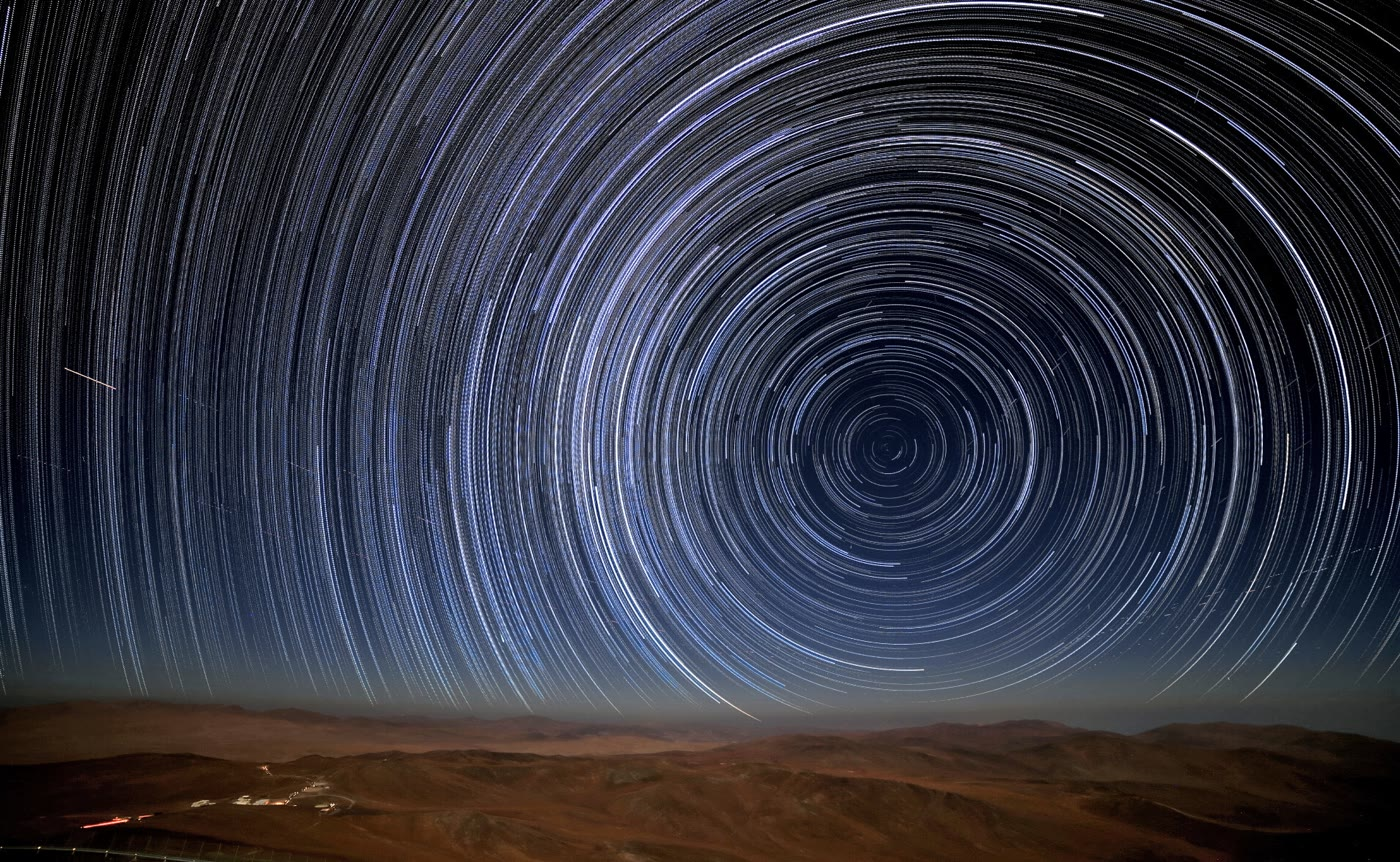
\includegraphics[width=0.8\linewidth]{images/book3/b1-star-trails-paranal.jpg}
% ledger: commons:eso-paranal-star-trails, mpc:paranal

{\small آثار النجوم فوق مرصد بارانال، في صحراء أتاكاما، عند \omterm{def:b1:spherical-astronomy:geographic}{العرض الجغرافي} \ang{24.6}~ج: يسجّل التعريض الطويل قوس كل نجم حول \omterm{def:b1:spherical-astronomy:celestial-sphere}{القطب السماوي} الجنوبي، الذي يقع على ارتفاع \ang{24.6} فوق الأفق الجنوبي. الصورة: R.~Wesson/ESO، بترخيص CC BY 4.0.}
\end{omfigure}

\section{الزمن النجمي والزمن الشمسي}

\begin{definition}[دائرة البروج]\label{def:b1:spherical-astronomy:ecliptic}
\emph{دائرة البروج}\index{دائرة البروج} هي \omterm{def:b1:spherical-astronomy:spherical-triangle}{الدائرة العظمى} من \omterm{def:b1:spherical-astronomy:celestial-sphere}{الكرة السماوية} التي تبدو عليها الشمس تسير في السنة، وهي أثر مستوى مدار الأرض. وهي مائلة على \omterm{def:b1:spherical-astronomy:celestial-sphere}{خط الاستواء السماوي} بزاوية \emph{ميل دائرة البروج}\index{ميل دائرة البروج} $\varepsilon$، وهي ميل محور الأرض على مدارها. وتتقاطع دائرة البروج مع خط الاستواء في نقطتين؛ و\emph{نقطة الاعتدال الربيعي}\index{نقطة الاعتدال الربيعي} $\gamma$ هي التي تعبرها الشمس صاعدةً نحو الشمال في مارس. وطول الشمس الفلكي $\lambda_\odot$ على دائرة البروج هو زاويتها على طول دائرة البروج من $\gamma$، مقيسةً شرقًا.
\end{definition}

% ledger: earth:obliquity (23.44)
\omterm{def:b1:spherical-astronomy:ecliptic}{ميل دائرة البروج} اليوم هو $\varepsilon = \ang{23.44}$.

\begin{definition}[الزمن النجمي]\label{def:b1:spherical-astronomy:sidereal-time}
\emph{الزمن النجمي}\index{الزمن النجمي} المحلي هو \omterm{def:b1:spherical-astronomy:equatorial}{الزاوية الساعية} \omterm{def:b1:spherical-astronomy:ecliptic}{لنقطة الاعتدال الربيعي} $\gamma$. واليوم النجمي هو الفاصل بين مرورين متتاليين للنقطة $\gamma$ بخط الزوال.
\end{definition}

لأن \omterm{def:b1:spherical-astronomy:equatorial}{المطلع المستقيم} يُقاس شرقًا من $\gamma$، \omterm{def:b1:spherical-astronomy:equatorial}{والزاوية الساعية} غربًا من خط الزوال، فإن كل نجم يحقق
\[
  H = \mathrm{LST} - \alpha ,
\]
حيث LST هو \omterm{def:b1:spherical-astronomy:sidereal-time}{الزمن النجمي} المحلي: يعبر النجم خط الزوال حين يساوي \omterm{def:b1:spherical-astronomy:sidereal-time}{الزمن النجمي} مطلعه المستقيم. وساعة المرصد التي تُظهر \omterm{def:b1:spherical-astronomy:sidereal-time}{الزمن النجمي} تبيّن في لمحة أيّ جزء من السماء يقع فوق الرأس.

\begin{proposition}[اليوم النجمي واليوم الشمسي]\label{prop:b1:spherical-astronomy:sidereal-day}
في \omterm{def:b1:spherical-astronomy:tropical-year}{السنة المدارية} التي تضم $N$ يومًا شمسيًا متوسطًا، تدور الأرض $N + 1$ دورة بالنسبة إلى النجوم. فيكون اليوم النجمي مساويًا
\[
  \frac{N}{N + 1}\times\qty{24}{h},
\]
ومع $N = 365.2422$ يكون ذلك \qty{23}{h}~\qty{56}{min}~\qty{4.09}{s}: فيعبر النجم خط الزوال كل يوم أبكر بمقدار \qty{3}{min}~\qty{56}{s} من \omterm{def:b1:spherical-astronomy:solar-time}{الزمن الشمسي المتوسط}.
\end{proposition}

\begin{proof}
% ledger: usno:tropical-year, earth:Trot (23.9345 h)
نحسب الدورات بالنسبة إلى الشمس وبالنسبة إلى النجوم خلال سنة واحدة. تتحرك الشمس دورةً واحدةً على \omterm{def:b1:spherical-astronomy:ecliptic}{دائرة البروج} شرقًا في السنة، في اتجاه دوران الأرض. فبالنسبة إلى الشمس تدور الأرض دورةً أقلّ مما تدور بالنسبة إلى النجوم، فيملأ $N$ يومًا شمسيًا و$N + 1$ يومًا نجميًا السنةَ نفسها. واليوم النجمي هو $N/(N+1)$ من اليوم الشمسي، أي $\qty{86400}{s}\times 365.2422/366.2422 = \qty{86164.09}{s}$؛ والفرق هو $\qty{235.9}{s}$. وهذا يوافق دورة الأرض بالنسبة إلى النجوم المقيسة، \qty{23.9345}{h}.
\end{proof}

\begin{definition}[الزمن الشمسي]\label{def:b1:spherical-astronomy:solar-time}
\emph{الزمن الشمسي الظاهري}\index{الزمن الشمسي الظاهري} هو \omterm{def:b1:spherical-astronomy:equatorial}{الزاوية الساعية} للشمس زائدًا 12 ساعة: فالمزولة تُظهره، ويكون الظهر حين تعبر الشمس خط الزوال. و\emph{الزمن الشمسي المتوسط}\index{الزمن الشمسي المتوسط} هو \omterm{def:b1:spherical-astronomy:equatorial}{الزاوية الساعية}، زائدًا 12 ساعة، لشمس وهمية متوسطة تسير على \omterm{def:b1:spherical-astronomy:celestial-sphere}{خط الاستواء السماوي} بسرعة منتظمة، فتتمّ دورتها في \omterm{def:b1:spherical-astronomy:tropical-year}{السنة المدارية}. وفرقهما، الظاهري ناقص المتوسط، هو \emph{معادلة الزمن}\index{معادلة الزمن}.
\end{definition}

وتسير الشمس الحقيقية أمام الشمس المتوسطة ثم خلفها لسببين. فالأرض تتحرك أسرع قرب الحضيض، في أوائل يناير، منها قرب الأوج، فيكون تقدّم الشمس على \omterm{def:b1:spherical-astronomy:ecliptic}{دائرة البروج} غير منتظم (قانون كبلر الثاني)؛ والشمس تسير على \omterm{def:b1:spherical-astronomy:ecliptic}{دائرة البروج}، وهي مائلة على خط الاستواء، فتُسقَط الحركة المنتظمة على \omterm{def:b1:spherical-astronomy:ecliptic}{دائرة البروج} على خط الاستواء الذي تقيسه \omterm{def:b1:spherical-astronomy:equatorial}{الزاوية الساعية} بتفاوت، أسرع قرب الانقلابين منها قرب الاعتدالين. وتحفظ الساعات المدنية \omterm{def:b1:spherical-astronomy:solar-time}{الزمن الشمسي المتوسط} على خط زوال مرجعي في منطقتها الزمنية؛ ويسبق الزمن المحلي المتوسط عند \omterm{def:b1:spherical-astronomy:geographic}{الطول الجغرافي} $\lambda$ الزمنَ في غرينتش بمقدار $\lambda/\ang{15}$ ساعة.

\begin{omfigure}
\begin{tikzpicture}
\begin{axis}[omrecord, width=0.9\linewidth, height=5.2cm, xmin=0, xmax=365,
  xtick={0,31,59,90,120,151,181,212,243,273,304,334,365},
  xticklabels={1,2,3,4,5,6,7,8,9,10,11,12,},
  xlabel={\foreignlanguage{arabic}{الشهر}}, ylabel={\foreignlanguage{arabic}{معادلة الزمن \babelsublr{(\unit{min})}}}, ymin=-20, ymax=21,
  tick label style={font=\scriptsize}, label style={font=\small}]
\addplot[black!50, line width=0.4pt] coordinates {(0,0) (365,0)};
\addplot[omDef, line width=1.1pt] table[x=day, y=eot_min] {figdata/out/bachelor-1-day_length-eot.dat};
\node[font=\scriptsize, above, fill=white, inner sep=1pt] at (axis cs:306,16.6) {$+16.4$};
\node[font=\scriptsize, below, fill=white, inner sep=1pt] at (axis cs:41,-14.4) {$-14.2$};
\end{axis}
\end{tikzpicture}

{\small \omterm{def:b1:spherical-astronomy:solar-time}{معادلة الزمن} على مدار السنة (الظاهري ناقص المتوسط): تتقدم المزولة حتى \qty{16.4}{min} في أوائل نوفمبر، وتتأخر \qty{14.2}{min} في منتصف فبراير. محسوبة من مدار كبلري بالاختلاف المركزي 0.0167 وميل \ang{23.44}، وخط طول الحضيض، وتاريخ اعتدال مارس 2026.}
% ledger: earth:ecc, earth:obliquity, nasa:earth-perihelion-longitude, usno:seasons-2026
\end{omfigure}

\section{الطلوع والغروب والشمس}

\begin{proposition}[الطلوع والغروب]\label{prop:b1:spherical-astronomy:rising}
عند \omterm{def:b1:spherical-astronomy:geographic}{العرض الجغرافي} $\varphi$، يطلع نجم ميله $\delta$ ويغرب، فيعبر الأفق عند الزاويتين الساعيتين $\pm H_0$ بحيث
\[
  \cos H_0 = -\tan\varphi\tan\delta ,
\]
وعند \omterm{def:b1:spherical-astronomy:horizontal}{السمت} $\mathrm{A}_0$ حيث $\cos\mathrm{A}_0 = \sin\delta/\cos\varphi$ (عند الطلوع، ويغرب عند $\ang{360} - \mathrm{A}_0$). ويبقى فوق الأفق مدة $2H_0$، محوَّلة إلى ساعات بمعدل \ang{15} في الساعة.
\end{proposition}

\begin{proof}
على الأفق يكون $h = 0$، و\cref{prop:b1:spherical-astronomy:transform} تعطي
$0 = \sin\varphi\sin\delta + \cos\varphi\cos\delta\cos H_0$، و$\cos\mathrm{A}_0 = \sin\delta/\cos\varphi$. وتزداد \omterm{def:b1:spherical-astronomy:equatorial}{الزاوية الساعية} بانتظام، بمقدار \ang{15} في الساعة، من $-H_0$ عند الطلوع إلى $+H_0$ عند الغروب.
\end{proof}

وبالنسبة إلى الشمس يعطي هذا طول النهار، إذا عُدّت الشمس نقطةً وأُهمل انكسار الضوء في الهواء (وكلاهما يضيف دقائق قليلة إلى ضوء النهار). وعند الاعتدالين يكون $\delta = 0$ و$H_0 = \ang{90}$: يدوم النهار والليل اثنتي عشرة ساعة في كل مكان، وتطلع الشمس من الشرق تمامًا.

\begin{omfigure}
\begin{tikzpicture}
\begin{axis}[omrecord, width=0.85\linewidth, height=5.6cm, xmin=40, xmax=320, ymin=0, ymax=75,
  xtick={45,90,135,180,225,270,315}, xticklabels={ش ق,ق,ج ق,ج,ج غ,غ,ش غ}, ytick={0,15,30,45,60,75},
  xlabel={\foreignlanguage{arabic}{السمت}}, ylabel={\foreignlanguage{arabic}{ارتفاع الشمس \babelsublr{($^\circ$)}}},
  tick label style={font=\scriptsize}, label style={font=\small}]
\addplot[omThm, line width=1pt] table[x=az_deg, y=alt_deg] {figdata/out/bachelor-1-sun_paths-june.dat};
\addplot[black, line width=1pt] table[x=az_deg, y=alt_deg] {figdata/out/bachelor-1-sun_paths-equinox.dat};
\addplot[omDef, line width=1pt] table[x=az_deg, y=alt_deg] {figdata/out/bachelor-1-sun_paths-december.dat};
\begin{scope}[font=\scriptsize, fill=white, fill opacity=0.8, text opacity=1, inner sep=1pt]
  \node[omThm, above, fill=white] at (axis cs:180,68.4) {انقلاب يونيو، $\ang{68.4}$};
  \node[above, fill=white] at (axis cs:180,45) {الاعتدالان، $\ang{45}$};
  \node[omDef, above, fill=white] at (axis cs:180,21.6) {انقلاب ديسمبر، $\ang{21.6}$};
\end{scope}
\end{axis}
\end{tikzpicture}

{\small مسار الشمس عبر السماء عند \omterm{def:b1:spherical-astronomy:geographic}{العرض الجغرافي} \ang{45}~ش: في انقلاب يونيو (بالأحمر)، وفي الاعتدالين (بالأسود)، وفي انقلاب ديسمبر (بالأزرق)، مع ارتفاعات الظهر $\ang{90} - \varphi + \delta_\odot$. وعند الاعتدالين تطلع الشمس من الشرق تمامًا وتغرب من الغرب تمامًا؛ وفي يونيو تطلع من الشمال الشرقي.}
\end{omfigure}

\begin{proposition}[ميل الشمس]\label{prop:b1:spherical-astronomy:sun-declination}
عندما تكون الشمس عند طول $\lambda_\odot$ على \omterm{def:b1:spherical-astronomy:ecliptic}{دائرة البروج}، يحقق ميلها ومطلعها المستقيم العلاقتين الآتيتين
\[
  \sin\delta_\odot = \sin\varepsilon\sin\lambda_\odot, \qquad
  \tan\alpha_\odot = \cos\varepsilon\tan\lambda_\odot .
\]
\end{proposition}

\begin{proof}
نأخذ المحاور بحيث يتّجه المحور $x$ نحو $\gamma$، ويتّجه المحور $z$ نحو \omterm{def:b1:spherical-astronomy:celestial-sphere}{القطب السماوي} الشمالي.
في محاور $x$ و$y'$ و$z'$ المرتبطة \omterm{def:b1:spherical-astronomy:ecliptic}{بدائرة البروج}، والمحور $z'$ نحو قطبها، يكون اتجاه الشمس
$(\cos\lambda_\odot, \sin\lambda_\odot, 0)$. ومحاور \omterm{def:b1:spherical-astronomy:ecliptic}{دائرة البروج} هي محاور خط الاستواء بعد أن تُدار بالزاوية $\varepsilon$ حول $x$، فيكون اتجاه الشمس في المحاور الاستوائية
$(\cos\lambda_\odot,\ \sin\lambda_\odot\cos\varepsilon,\
\sin\lambda_\odot\sin\varepsilon)$. ومركبته $z$ هي $\sin\delta_\odot$؛
ونسبة مركبتي $y$ و$x$ هي $\tan\alpha_\odot$.
\end{proof}

\begin{omfigure}
\begin{tikzpicture}
\begin{axis}[omrecord, width=0.9\linewidth, height=6cm, xmin=0, xmax=365, ymin=0, ymax=24,
  xtick={0,31,59,90,120,151,181,212,243,273,304,334,365},
  xticklabels={1,2,3,4,5,6,7,8,9,10,11,12,}, ytick={0,6,12,18,24},
  ylabel={\foreignlanguage{arabic}{طول النهار \babelsublr{(\unit{h})}}}, tick label style={font=\scriptsize}, label style={font=\small},
  legend style={font=\scriptsize, at={(0.5,1.02)}, anchor=south, draw=none}, legend columns=5,
  legend cell align=left]
\addplot[black, line width=0.9pt] table[x=day, y=lat0] {figdata/out/bachelor-1-day_length-lengths.dat};
\addplot[omDef, line width=0.9pt] table[x=day, y=lat30] {figdata/out/bachelor-1-day_length-lengths.dat};
\addplot[omThm, line width=0.9pt] table[x=day, y=lat45] {figdata/out/bachelor-1-day_length-lengths.dat};
\addplot[omField, line width=0.9pt] table[x=day, y=lat60] {figdata/out/bachelor-1-day_length-lengths.dat};
\addplot[black, line width=0.9pt, densely dashed] table[x=day, y=lat70] {figdata/out/bachelor-1-day_length-lengths.dat};
\legend{{\mbox{\textdir TLT \ang{0}}}, {\mbox{\textdir TLT \ang{30}}~ش}, {\mbox{\textdir TLT \ang{45}}~ش}, {\mbox{\textdir TLT \ang{60}}~ش}, {\mbox{\textdir TLT \ang{70}}~ش}}
\end{axis}
\end{tikzpicture}

{\small طول النهار (مركز قرص الشمس فوق الأفق الهندسي) على مدار السنة عند خمسة أعراض شمالية، انطلاقًا من \cref{prop:b1:spherical-astronomy:rising,prop:b1:spherical-astronomy:sun-declination}. وعند \ang{70}~ش تبقى الشمس فوق الأفق أسابيع حول انقلاب يونيو، وتبقى تحته حول انقلاب ديسمبر. وفي نصف الكرة الجنوبي تتزحزح المنحنيات نصف سنة.}
\end{omfigure}

\begin{definition}[الإشماس]\label{def:b1:spherical-astronomy:insolation}
\emph{الإشماس}\index{الإشماس} في مكان ولحظة معيّنين هو قدرة ضوء الشمس الساقط على وحدة المساحة من سطح أفقي عند أعلى الغلاف الجوي. فإذا كان $S_0$ الإشعاع الشمسي عند المسافة المتوسطة $a$ للشمس، و$r$ المسافة الفعلية، و$\theta_z$ البعد الزاوي للشمس عن \omterm{def:b1:spherical-astronomy:celestial-sphere}{سمت الرأس}،
\[
  I = S_0\left(\frac{a}{r}\right)^{2}\cos\theta_z = S_0\left(\frac{a}{r}\right)^{2}\sin h_\odot
  \quad (h_\odot > 0), \qquad I = 0 \text{ ليلًا}.
\]
\end{definition}

% ledger: earth:TSI (1361 W/m2), earth:peri, earth:aph, earth:a
العامل $(a/r)^2$ هو قانون التربيع العكسي للضوء (كتب الفيزياء)؛ والعامل $\cos\theta_z$ يظهر لأن حزمة مقطعها متر مربع واحد تنتشر على $1/\cos\theta_z$ متر مربع من الأرض الأفقية. ومع $S_0 = \qty{1361}{W.m^{-2}}$ والمسافة بين الشمس والأرض بين \qty{147.1e6}{km} عند الحضيض و\qty{152.1e6}{km} عند الأوج، يتغيّر العامل $(a/r)^2$ بمقدار $\pm\qty{3.4}{\percent}$ في السنة. أما ميل المحور فيفعل أكثر من ذلك بكثير: إذ يغيّر \omterm{def:b1:spherical-astronomy:horizontal}{ارتفاع الظهر} ومدة النهار معًا، وهذان معًا يصنعان الفصول. ومجموع \omterm{def:b1:spherical-astronomy:insolation}{الإشماس} اليومي والسنوي، الذي يحرّك المناخ، يُحسب في \cref{ch:b1:radiation-heat-transport}.


\section{التقاويم}

\begin{definition}[السنة المدارية]\label{def:b1:spherical-astronomy:tropical-year}
\emph{السنة المدارية}\index{السنة المدارية} هي الفاصل المتوسط بين مرورين متتاليين للشمس \omterm{def:b1:spherical-astronomy:ecliptic}{بنقطة الاعتدال الربيعي}. وهي التي تضبط الفصول، وتدوم 365.2422 يومًا شمسيًا متوسطًا.
\end{definition}

% ledger: usno:tropical-year, earth:Psid (365.256 d)
\omterm{def:b1:spherical-astronomy:tropical-year}{والسنة المدارية} أقصر بنحو عشرين دقيقة من السنة النجمية، وهي الزمن الذي تعود فيه الأرض إلى الموضع نفسه بين النجوم (365.256 يومًا)، لأن محور الأرض يدور ببطء، فيتقدّم، ويحمل نقطة الاعتدال إلى الوراء على \omterm{def:b1:spherical-astronomy:ecliptic}{دائرة البروج} (الكتاب 2). ويجب أن يضم التقويم عددًا صحيحًا من الأيام في \omterm{def:b1:spherical-astronomy:tropical-year}{السنة المدارية}، حتى تعود الفصول إلى التواريخ نفسها.

\begin{proposition}[التقويم الغريغوري]\label{prop:b1:spherical-astronomy:gregorian}
في التقويم الغريغوري تكون السنة كبيسة من 366 يومًا إذا كان عددها قابلًا للقسمة على 4، إلا سنوات القرون فلا تكون كبيسة إلا إذا قبلت القسمة على 400. ومتوسط السنة فيه
\[
  365 + \frac14 - \frac1{100} + \frac1{400} = \num{365.2425}\text{ يومًا},
\]
ويتباعد عن الفصول بيوم واحد في نحو 3300 سنة.
\end{proposition}

\begin{proof}
% ledger: usno:leap-rule, usno:tropical-year
في 400 سنة توجد 100 سنة قابلة للقسمة على 4، من بينها أربع سنوات قرنية، ثلاث منها غير قابلة للقسمة على 400. فتكون 97 سنة كبيسة، و$400\times 365 + 97 = 146\,097$ يومًا، أي 365.2425 يومًا في السنة. وبالنسبة إلى \omterm{def:b1:spherical-astronomy:tropical-year}{السنة المدارية} البالغة 365.2422 يومًا يكون الفائض 0.0003 يوم في السنة: يومًا واحدًا في $1/0.0003 \approx 3300$ سنة.
\end{proof}

\begin{history}[إصلاح التقويم عام 1582]
% ledger: usno:gregorian-1582
كان تقويم يوليوس، الموروث من روما، يضيف يومًا كبيسة كل أربع سنين: فسنته البالغة 365.25 يومًا أطول من \omterm{def:b1:spherical-astronomy:tropical-year}{السنة المدارية} بمقدار 0.0078 يوم، أي بيوم كل 128 سنة. ومع توالي القرون انزاح تاريخ الاعتدال الربيعي عن 21 مارس، وهو التاريخ الذي كان حساب عيد الفصح يعتمد عليه. وفي 1582 قدّم البابا غريغوريوس الثالث عشر التقويم الذي يحمل اسمه، فأسقط الأيام المتراكمة دفعةً واحدة، واستبدل بقاعدة يوليوس قاعدة \cref{prop:b1:spherical-astronomy:gregorian}. وقد صار التقويم المدني المعترَف به دوليًا.
\end{history}

\begin{inthefield}[تحديد الموقع بالنجوم]
قبل تحديد المواقع بالأقمار الصناعية، كان الملاحون في البحر يحدّدون عرضهم الجغرافي وطولهم الجغرافي من السماء. فبالسكستانت كانوا يقيسون \omterm{def:b1:spherical-astronomy:horizontal}{ارتفاع الشمس} عند الظهر، أو ارتفاع نجمين أو ثلاثة عند الغسق، ويقرؤون الوقت على كرونومتر مضبوط على زمن خط زوال غرينتش. وكل ارتفاع، مع \omterm{def:b1:spherical-astronomy:equatorial}{ميل النجم} وزاويته الساعية في غرينتش من التقويم الفلكي، يعطي دائرةً صغرى على الأرض تقع عليها السفينة، وهي دائرة النقاط التي يكون النجم عندها على ذلك \omterm{def:b1:spherical-astronomy:horizontal}{الارتفاع}. وتتقاطع دائرتان أو ثلاث من هذه الدوائر عند موقع السفينة، فهي مثلثات كروية تُحلّ في البحر كل يوم. أما \omterm{def:b1:spherical-astronomy:horizontal}{ارتفاع الشمس} عند الظهر وحده فيعطي \omterm{def:b1:spherical-astronomy:geographic}{العرض الجغرافي} (\cref{prop:b1:spherical-astronomy:culmination})؛ وأما زمن الظهر المحلي على الساعة فيعطي \omterm{def:b1:spherical-astronomy:geographic}{الطول الجغرافي}، بمعدل أربع دقائق زمنية لكل درجة.
\begin{center}
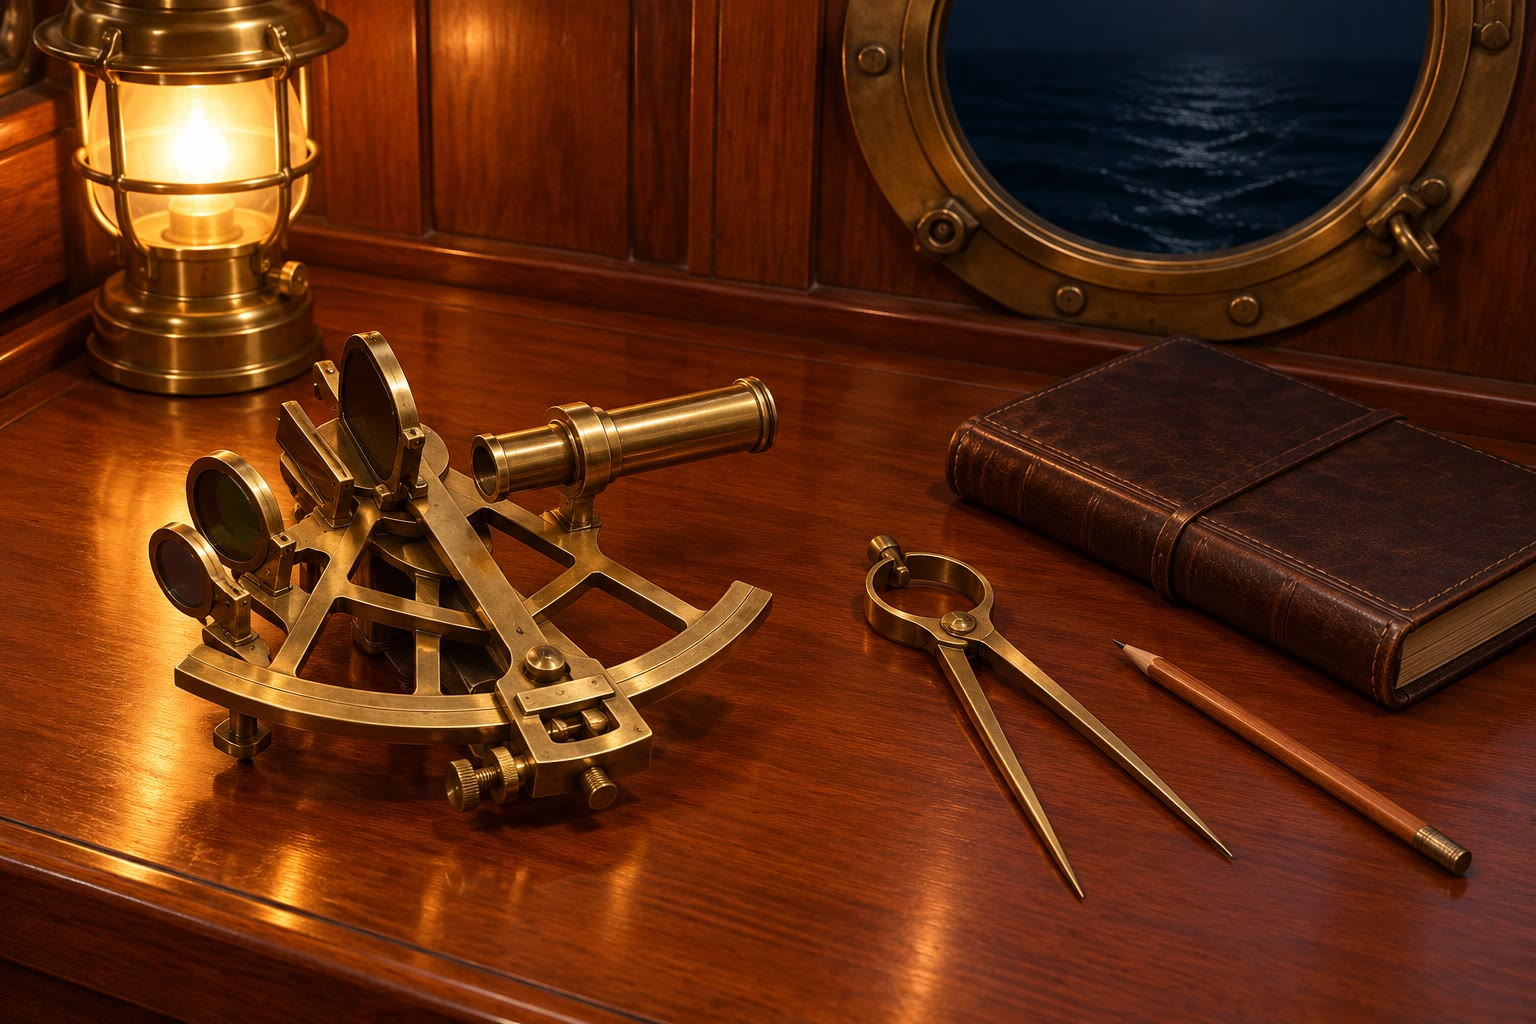
\includegraphics[width=0.55\linewidth]{images/book3/ai/b1-sextant.jpg}
\end{center}
\end{inthefield}

\section{التمارين}

\begin{exercise}[$\star$]\label{exo:b1:spherical-astronomy:1}
يقع راصد عند \omterm{def:b1:spherical-astronomy:geographic}{العرض الجغرافي} \ang{52}~ش. على أيّ ارتفاع يقع \omterm{def:b1:spherical-astronomy:celestial-sphere}{القطب السماوي} الشمالي؟ وأيّ النجوم، بحسب ميلها، لا تغيب أبدًا هناك، وأيّها لا تطلع أبدًا؟
\end{exercise}

\begin{exercise}[$\star$]\label{exo:b1:spherical-astronomy:2}
حوّل مطلعًا مستقيمًا قدره \qty{6}{h}~\qty{45}{min} إلى درجات. وعند زمن نجمي محلي قدره \qty{10}{h}~\qty{0}{min}، احسب \omterm{def:b1:spherical-astronomy:equatorial}{الزاوية الساعية} لنجم له هذا \omterm{def:b1:spherical-astronomy:equatorial}{المطلع المستقيم}. أيقع النجم شرق خط الزوال أم غربه؟
\end{exercise}

\begin{exercise}[$\star$]\label{exo:b1:spherical-astronomy:3}
عند \omterm{def:b1:spherical-astronomy:geographic}{العرض الجغرافي} \ang{40}~ش، احسب \omterm{def:b1:spherical-astronomy:horizontal}{ارتفاع الشمس} عند الظهر في الانقلابين وفي الاعتدالين ($\varepsilon = \ang{23.44}$).
\end{exercise}

\begin{exercise}[$\star$]\label{exo:b1:spherical-astronomy:4}
هل كانت سنة 1900 كبيسة؟ وهل كانت 2000؟ وهل ستكون 2100؟ وبكم يومًا في القرن يتباعد تقويم يوليوس عن سنة مدارية مقدارها 365.2422 يومًا، وبكم يومًا يتباعد التقويم الغريغوري؟
\end{exercise}

\begin{exercise}[$\star\star$]\label{exo:b1:spherical-astronomy:5}
تقع نقطتان على \omterm{def:b1:spherical-astronomy:geographic}{العرض الجغرافي} \ang{45}~ش، عند الطولين \ang{0} و\ang{90}~ق. احسب المسافة على \omterm{def:b1:spherical-astronomy:spherical-triangle}{الدائرة العظمى} بينهما ($R = \qty{6371}{km}$)، والمسافة على دائرة عرضهما. أيّهما أقصر، وبكم؟
\end{exercise}

\begin{exercise}[$\star\star$]\label{exo:b1:spherical-astronomy:6}
عند \omterm{def:b1:spherical-astronomy:geographic}{العرض الجغرافي} \ang{48}~ش، لنجم ميله \ang{20} زاويته الساعية \ang{30}. احسب ارتفاعه وسمته. في أيّ اتجاه ينبغي أن ينظر الراصد؟
\end{exercise}

\begin{exercise}[$\star\star$]\label{exo:b1:spherical-astronomy:7}
احسب طول النهار عند \omterm{def:b1:spherical-astronomy:geographic}{العرض الجغرافي} \ang{60}~ش في انقلاب يونيو، مع اعتبار الشمس نقطةً على أفق هندسي. وتحقّق من جوابك على شكل طول النهار.
\end{exercise}

\begin{exercise}[$\star\star$]\label{exo:b1:spherical-astronomy:8}
يعبر نجم خط الزوال الليلة عند الساعة 22:00 من الزمن المحلي المتوسط. في أيّ ساعة سيعبره بعد 30 يومًا؟ وبعد كم يومًا سيعبره عند الظهر، فيكون غير مرئي في ضوء النهار؟
\end{exercise}

\begin{exercise}[$\star\star$]\label{exo:b1:spherical-astronomy:9}
احسب \omterm{def:b1:spherical-astronomy:insolation}{الإشماس} عند أعلى الغلاف الجوي عند الظهر، على \omterm{def:b1:spherical-astronomy:geographic}{العرض الجغرافي} \ang{45}~ش: (أ) في أحد الاعتدالين، آخذًا $r = a$؛ (ب) في انقلاب يونيو، آخذًا لقيمة $r$ مسافة الأوج. المعطيات: $S_0 = \qty{1361}{W.m^{-2}}$،
$a = \qty{149.598e6}{km}$، والأوج \qty{152.100e6}{km}.
\end{exercise}

\begin{exercise}[$\star\star\star$]\label{exo:b1:spherical-astronomy:10}
باستعمال \cref{prop:b1:spherical-astronomy:sun-declination}، احسب \omterm{def:b1:spherical-astronomy:equatorial}{ميل الشمس} ومطلعها المستقيم عندما يكون طولها على \omterm{def:b1:spherical-astronomy:ecliptic}{دائرة البروج} \ang{60}. وبكم درجة يتأخر \omterm{def:b1:spherical-astronomy:equatorial}{المطلع المستقيم} عن الطول؟ وفسّر بهذه النتيجة لماذا يسهم \omterm{def:b1:spherical-astronomy:ecliptic}{ميل دائرة البروج} في \omterm{def:b1:spherical-astronomy:solar-time}{معادلة الزمن}.
\end{exercise}

\begin{exercise}[$\star\star\star$]\label{exo:b1:spherical-astronomy:11}
بيّن أنه في انقلاب يونيو تطلع الشمس عند \omterm{def:b1:spherical-astronomy:horizontal}{السمت} $\mathrm{A}_0$ حيث $\cos\mathrm{A}_0 = \sin\varepsilon/\cos\varphi$. وعند أيّ \omterm{def:b1:spherical-astronomy:geographic}{عرض جغرافي} تطلع تمامًا في الشمال الشرقي؟ وماذا يحدث للصيغة عند أعراض أكبر من $\ang{90} - \varepsilon$؟
\end{exercise}

\begin{exercise}[$\star\star\star$]\label{exo:b1:spherical-astronomy:12}
الهلالة الكروية هي الجزء من الكرة المحصور بين نصفي دائرتين عظميين يصلان نقطتين متقابلتين، وبينهما الزاوية $\theta$. (أ) بيّن أن مساحتها هي $2\theta R^2$. (ب) كل ضلع من \omterm{def:b1:spherical-astronomy:spherical-triangle}{المثلث الكروي} $ABC$، إذا مُدّ إلى دائرة عظمى كاملة، يعطي مع الأضلاع الأخرى ثلاثة أزواج من الهلالات المتقابلة زواياها $A$ و$B$ و$C$ تغطي الكرة، فيكون المثلث ومقابله مغطّيين ثلاث مرات. استنتج مبرهنة جيرار: مساحة المثلث هي $R^2(A + B + C - \pi)$. (ج) طبّقها على المثلث الذي زواياه قائمة الثلاث، وعلى المثلث المرسوم في هذا الفصل (زواياه \ang{89.9} و\ang{64.9} و\ang{67.4}).
\end{exercise}

\section{مسألة: ليلة في مرصد جبلي}

\begin{problem}[{مسألة نهاية الأسبوع --- أين يقع مرصد بارانال، وماذا تُظهر سماؤه، وكم يطول أطول ليل فيه}]
\label{pb:b1:spherical-astronomy:1}
% ledger: mpc:paranal, mpc:greenwich, simbad:sirius, simbad:canopus, usno:seasons-2026, earth:obliquity, usno:tropical-year
% numbers computed in the scratch calculator calc/ch01.py from the rounded data
يقع مرصد بارانال في صحراء أتاكاما عند \omterm{def:b1:spherical-astronomy:geographic}{العرض الجغرافي} \ang{24.63}~ج \omterm{def:b1:spherical-astronomy:geographic}{والطول الجغرافي} \ang{70.40}~غ. ومرصد غرينتش الملكي، الذي تُعدّ منه الأطوال الجغرافية، يقع عند العرض \ang{51.48}~ش وعند الطول \ang{0.00}. ولنجمين لامعين في السماء الجنوبية الإحداثياتُ الآتية:
\begin{center}
\small
\begin{tabular}{lcc}
\hline
النجم & \omterm{def:b1:spherical-astronomy:equatorial}{المطلع المستقيم} & \omterm{def:b1:spherical-astronomy:equatorial}{الميل} \\
\hline
سيريوس & \mbox{\textdir TLT \qty{6}{h}~\qty{45}{min}~\qty{9}{s}} & \mbox{\textdir TLT \ang{-16.72}} \\
كانوبس & \mbox{\textdir TLT \qty{6}{h}~\qty{23}{min}~\qty{57}{s}} & \mbox{\textdir TLT \ang{-52.70}} \\
\hline
\end{tabular}
\end{center}
وخذ $R = \qty{6371}{km}$ و$\varepsilon = \ang{23.44}$ \omterm{def:b1:spherical-astronomy:tropical-year}{والسنة المدارية} 365.2422 يومًا، واعتبر الشمس نقطةً على أفق هندسي.

\medskip
\noindent\textbf{الجزء الأول --- بارانال على الكرة الأرضية.}
\begin{enumerate}
  \item أعطِ متممَي العرض لبارانال ولغرينتش، وفرقَ \omterm{def:b1:spherical-astronomy:geographic}{الطول الجغرافي} بينهما.
  \item اكتب قاعدة جيب التمام للمثلث الذي رؤوسه القطب الشمالي وبارانال وغرينتش، واحسب جيب تمام البعد الزاوي $\Delta$ بين المرصدين.
  \item استنتج $\Delta$ بالدرجات، والمسافة على \omterm{def:b1:spherical-astronomy:spherical-triangle}{الدائرة العظمى} بالكيلومترات.
  \item احسب الاتجاه الابتدائي من بارانال نحو غرينتش (\cref{met:b1:spherical-astronomy:great-circle}).
  \item تحقّق من الاتجاه بقاعدة الجيب.
  \item هل تصل طائرة تحافظ على هذا الاتجاه طوال الرحلة إلى غرينتش؟ علّل.
\end{enumerate}

\medskip
\noindent\textbf{الجزء الثاني --- سماء بارانال.}
\begin{enumerate}[resume]
  \item على أيّ ارتفاع يقع \omterm{def:b1:spherical-astronomy:celestial-sphere}{القطب السماوي} الجنوبي فوق الأفق الجنوبي لبارانال؟
  \item على أيّ ارتفاع يعبر سيريوس خط الزوال، وعلى أيّ جانب من \omterm{def:b1:spherical-astronomy:celestial-sphere}{سمت الرأس}؟
  \item دون أيّ ميل يكون النجم دائرًا حول القطب في بارانال؟ وهل كانوبس نجم دائر حول القطب؟
  \item ما أعلى ارتفاع يبلغه كانوبس؟
  \item احسب \omterm{def:b1:spherical-astronomy:equatorial}{الزاوية الساعية} التي يطلع عندها سيريوس، وكم يبقى فوق الأفق بالساعات النجمية.
  \item على أيّ سمت يطلع سيريوس؟
\end{enumerate}

\medskip
\noindent\textbf{الجزء الثالث --- الساعات.}
\begin{enumerate}[resume]
  \item ما \omterm{def:b1:spherical-astronomy:sidereal-time}{الزمن النجمي} المحلي عندما يعبر سيريوس خط الزوال؟
  \item احسب طول اليوم النجمي، وبكم دقيقة يتقدّم عبور النجم خط الزوال كل ليلة.
  \item خذ \omterm{def:b1:spherical-astronomy:sidereal-time}{الزمن النجمي} المحلي عند منتصف الليل المحلي المتوسط مساويًا \qty{12}{h} في اعتدال مارس (20 مارس 2026)، حين تكون الشمس قرب \omterm{def:b1:spherical-astronomy:ecliptic}{نقطة الاعتدال الربيعي}؛ ثم يكسب \omterm{def:b1:spherical-astronomy:sidereal-time}{الزمن النجمي} $24/365.2422$ ساعة كل يوم. بعد كم يومًا من الاعتدال يعبر سيريوس خط الزوال عند منتصف الليل المحلي المتوسط؟ وفي أيّ تاريخ؟
  \item في تلك الليلة، بكم يختلف الزمن المحلي المتوسط في بارانال عن الزمن في غرينتش؟
  \item تبلغ \omterm{def:b1:spherical-astronomy:solar-time}{معادلة الزمن} عندئذٍ نحو \qty{-3}{min}. ما الوقت الذي تُظهره مزولة في المرصد (\omterm{def:b1:spherical-astronomy:solar-time}{الزمن الشمسي الظاهري}) عندما يعبر سيريوس خط الزوال؟
  \item بكم يتقدّم عبوره بعد أسبوع؟
\end{enumerate}

\medskip
\noindent\textbf{الجزء الرابع --- أطول ليل.}
\begin{enumerate}[resume]
  \item ما \omterm{def:b1:spherical-astronomy:equatorial}{ميل الشمس} في كلّ انقلاب؟
  \item احسب \omterm{def:b1:spherical-astronomy:horizontal}{ارتفاع الشمس} عند الظهر في بارانال في انقلابي يونيو وديسمبر. على أيّ جانب من \omterm{def:b1:spherical-astronomy:celestial-sphere}{سمت الرأس} تكون في ديسمبر؟
  \item في انقلاب ديسمبر تبلغ المسافة بين الشمس والأرض 0.9837 من المسافة المتوسطة. احسب \omterm{def:b1:spherical-astronomy:insolation}{الإشماس} عند الظهر في أعلى الغلاف الجوي فوق بارانال ($S_0 = \qty{1361}{W.m^{-2}}$).
  \item في أيّ انقلاب يكون الليل أطول في بارانال؟ واحسب \omterm{def:b1:spherical-astronomy:equatorial}{الزاوية الساعية} لغروب الشمس في ذلك التاريخ.
  \item على أيّ سمت تطلع الشمس في ذلك التاريخ؟
  \item استنتج طول أطول ليل في السنة في بارانال، بالساعات والدقائق.
\end{enumerate}
\end{problem}
